\documentclass{article}

\usepackage[english]{babel}
\usepackage[a4paper,top=2cm,bottom=2cm,left=3cm,right=3cm,marginparwidth=1.75cm]{geometry}

\usepackage{amsthm}
\usepackage{amsmath}
\usepackage{graphicx}
\usepackage[table]{xcolor}
%\usepackage{soul}% highlight
\usepackage{svg}
\usepackage[normalem]{ulem}

\usepackage{csquotes}% fix warning
\usepackage[style=alphabetic,sorting=ndt]{biblatex}
\addbibresource{sources.bib}

\usepackage{float}% [H] on figures
\usepackage{placeins}% \FloatBarrier - do not have floats interrupting references
\usepackage{booktabs}% better tables
\usepackage{marginnote}% parentheticals on the side
% \usepackage{subcaption}% subfloats

\usepackage{tikz}
\usetikzlibrary{matrix, positioning}

\title{Pentomino Pathfinding}
\author{Steven Nguyen (icecream17)}

% pentomino colors
\definecolor{colorI}{HTML}{EEAAAA}
\definecolor{colorF}{HTML}{DDBB99}
\definecolor{colorL}{HTML}{CCCC88}
\definecolor{colorP}{HTML}{BBDD99}
\definecolor{colorN}{HTML}{AAEEAA}
\definecolor{colorT}{HTML}{99DDBB}
\definecolor{colorU}{HTML}{88CCCC}
\definecolor{colorV}{HTML}{99BBDD}
\definecolor{colorW}{HTML}{AAAAEE}
\definecolor{colorX}{HTML}{BB99DD}
\definecolor{colorY}{HTML}{CC88CC}
\definecolor{colorZ}{HTML}{DD99BB}

% tetromino colors
% = colorU
\definecolor{color4I}{HTML}{88CCCC}
% = colorL
\definecolor{color4O}{HTML}{CCCC88}

\definecolor{colorSecondary}{HTML}{440044}

% commands for pentominoes, to avoid needing to do "\@"
% as a bonus this highlights them and clarifies that they are a pentomino
\newcommand{\pentI}{\smash{\colorbox{colorI!50}{I}}}
\newcommand{\pentF}{\smash{\colorbox{colorF!50}{F}}}% it fits AAA contrast a11y but still,
\newcommand{\pentL}{\smash{\colorbox{colorL!50}{L}}}% 50% lighter for even further clarity
\newcommand{\pentP}{\smash{\colorbox{colorP!50}{P}}}
\newcommand{\pentN}{\smash{\colorbox{colorN!50}{N}}}
\newcommand{\pentT}{\smash{\colorbox{colorT!50}{T}}}
\newcommand{\pentU}{\smash{\colorbox{colorU!50}{U}}}
\newcommand{\pentV}{\smash{\colorbox{colorV!50}{V}}}
\newcommand{\pentW}{\smash{\colorbox{colorW!50}{W}}}
\newcommand{\pentX}{\smash{\colorbox{colorX!50}{X}}}
\newcommand{\pentY}{\smash{\colorbox{colorY!50}{Y}}}
\newcommand{\pentZ}{\smash{\colorbox{colorZ!50}{Z}}}

% place at end
\usepackage[colorlinks=true, allcolors=blue]{hyperref}

% place after hyperref; exception
\usepackage[capitalize,noabbrev,english]{cleveref}% english option is recommended in the Non-Bugs section

% place newtheorem after cleveref, for proper detection

% \theoremstyle{plain} % default
\theoremstyle{definition}% not semantic, but removes italics
\newtheorem{theorem}{Theorem}[section]
\newtheorem{corollary}[theorem]{Corollary}% Corollaries and examples are not necessarily of the previous theorem. A subcounter can be used to eliminate a different bug.
\newtheorem{lemma}[theorem]{Lemma}

\newtheorem{definition}[theorem]{Definition}
\newtheorem{property}[theorem]{Property}
\newtheorem{example}[theorem]{Example}

% \theoremstyle{remark}% not semantic to not have this, but keeps bold
\newtheorem*{conclusion}{Conclusion}
\newtheorem*{note}{Note}

\newcommand{\minordetail}[1]{\textcolor{gray}{#1}}
\newcommand{\newterm}[1]{\textit{#1}}
\newcommand{\badterm}[1]{\textcolor{red}{\uwave{\textcolor{black}{#1}}}}

% DeclareMathOperator but more simple
\newcommand{\adj}{\operatorname{adj}}
\newcommand{\holes}{\operatorname{holes}}
\newcommand{\border}{\operatorname{border}}
\newcommand{\bound}{\operatorname{bound}}
\newcommand{\caves}{\operatorname{caves}}
\newcommand{\outside}{\operatorname{outside}}

\begin{document}
\maketitle

% \begin{abstract}
% Your abstract.
% \end{abstract}

\tableofcontents





\section{Introduction}

This paper will try to solve the Pentomino Pathfinding problem for various rectangular grids. See \cite{v1} and \cite{v2} for further introduction.

\cite{v1} posed the following problem: Given a rectangular $n \times m$ grid of squares, place a subset of the twelve pentominoes (\cref{fig:pentominoes}), and endpoints $A$ and $B$ on the grid \minordetail{without overlaps} such that $\#_{n, m}$ = the length of (the shortest path \minordetail{of nonempty, orthogonal squares} from $A$ to $B$) is maximized.

The maximum length given some placements $p$ is denoted by $\#^{p}_{n, m}$; independently, when $n = m$, the row and column indices are collapsed: $\#_n$.

\begin{figure}[htbp]
    \centering
    \includesvg[width=0.5\linewidth]{All_18_Pentominoes.svg}
    \caption{The twelve pentominoes and their reflections \cite{pentominoes};
    from left-to-right they are named \pentI, \pentF, \pentL, \pentP, \pentN,
    \pentT, \pentU, \pentV, \pentW, \pentX, \pentY, \pentZ, where
    \pentF, \pentL, \pentP, \pentN, \pentY, \pentZ{} are chiral
    and have their reflections shown.}
    \label{fig:pentominoes}
\end{figure}






\section{No pentominoes}

For $n$ = 1 and 2, $n \times n < 5$, so no pentomino can fit.
For $n$ = 3, 9 squares minus a pentomino is 4 squares, so the length 5 path is optimal. (\Cref{fig:no123})

\begin{figure}[htbp]
    \centering
    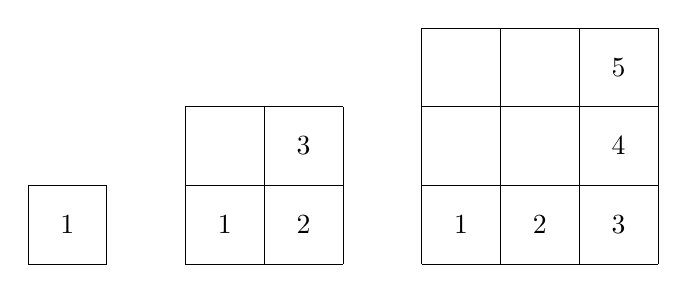
\begin{tikzpicture}
        \draw[step=1cm,black,very thin] (0,0) grid (1,1);
        \draw (0.5,0.5) node{1};

        \draw[step=1cm,black,very thin] (2,0) grid (4,2);
        \draw (2.5,0.5) node{1};
        \draw (3.5,0.5) node{2};
        \draw (3.5,1.5) node{3};

        \draw[step=1cm,black,very thin] (5,0) grid (8,3);
        \draw (5.5,0.5) node{1};
        \draw (6.5,0.5) node{2};
        \draw (7.5,0.5) node{3};
        \draw (7.5,1.5) node{4};
        \draw (7.5,2.5) node{5};
    \end{tikzpicture}
    \caption{$\#_1 = 1, \#_2 = 3, \#_3 = 5$ \cite{v1}}
    \label{fig:no123}
\end{figure}

Similar reasoning holds for $n = 2$, $m \le 6$: there is a path of length $m + 1 \le 7$, while $2m - 5 \le m + 1 \le 7$, so you cannot do any better than placing nothing. It turns out there is enough room for the I~piece, and so for $m = 6$ there are two solutions ignoring symmetry:

\begin{figure}[htbp]
    \centering
    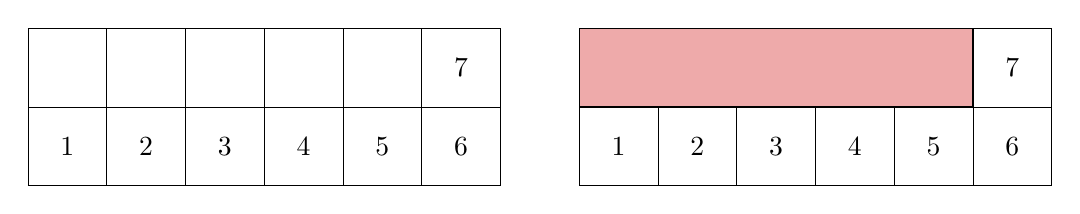
\begin{tikzpicture}
        \draw[step=1cm,black,very thin] (0,0) grid (6,2);
        \draw (0.5,0.5) node{1};
        \draw (1.5,0.5) node{2};
        \draw (2.5,0.5) node{3};
        \draw (3.5,0.5) node{4};
        \draw (4.5,0.5) node{5};
        \draw (5.5,0.5) node{6};
        \draw (5.5,1.5) node{7};

        \draw[step=1cm,black,very thin] (7,0) grid (13,2);
        \draw (7.5,0.5) node{1};
        \draw (8.5,0.5) node{2};
        \draw (9.5,0.5) node{3};
        \draw (10.5,0.5) node{4};
        \draw (11.5,0.5) node{5};
        \draw (12.5,0.5) node{6};
        \draw (12.5,1.5) node{7};
        \filldraw[fill=colorI] (7,1) rectangle (12,2);
    \end{tikzpicture}
    \label{fig:no2x5}
\end{figure}

\begin{definition}[Adjacency]
Two squares are \newterm{adjacent} iff they are one square diagonally or orthogonally apart. Two squares are \newterm{orthogonal} iff they are adjacent but not diagonally so. Two sets of squares $S$ and $T$ are \newterm{adjacent} if there is a pair of squares $(s, t) \in S \times T$ (Cartesian product) such that $s$ and $t$ are adjacent. The squares adjacent to a set of squares $S$ is denoted $\adj(S)$.
\end{definition}

\begin{definition}[Subgrid]
A subgrid is any connected subgraph of empty squares \minordetail{of the grid}. \minordetail{A square is empty iff it is does not have a pentomino.}
\end{definition}

\begin{definition}[Platter]
A \newterm{platter} is a (set of adjacent squares) not adjacent to another square.\marginnote{I don't use the term ``shape'' because two squares diagonally adjacent doesn't usually match people's intuitions.}% For this definition, the outside wall is considered a cycle of squares and can be part of the platter. (Doesn't work because holes and caves and convex)
\end{definition}

\begin{definition}[Outside]
For a platter $P$, $\outside(P)$ = All squares reachable from the wall or other platters
\end{definition}

\begin{definition}[Border]
A platter's \newterm{border} is the squares adjacent to the platter that are outside of it. $\border(P) = \adj(P) \cap \outside(P)$

If a platter cuts the grid into subgrids, we may restrict the outside to squares reachable from just that subgrid $s$. This is denoted $\border(P)_s$
\end{definition}

\begin{lemma}[Border removal]
\label{lem:Border removal}

Say we have a platter $p_1$ with the following properties:

\begin{enumerate}
\item $\border(p_1) = \adj(p_1)$
\item choosing any two squares on its border $A$ and $B$ where there is a path from $A$ to $B$, the shortest such path and the shortest such path upon removing the platter are the same length.
\end{enumerate}

Then the platter may be removed: $\#^{p}_{n, m} \le \#^{p - p_1}_{n, m}$
\end{lemma}

\begin{proof}
Can any preexisting path get shorter by entering the platter? No. Any preexisting path starts and ends outside the platter, by property 1. If the path wants to enter the platter, it must reach its border, go inside, then exit from another square on the border. But by property 2, going \emph{along} the border is at least as efficient.

So, any preexisting paths determining $\#^{p}_{n, m}$ will never enter the area where the platter disappeared from; i.e, such paths will not get shorter with the removal of the platter.
\end{proof}

\begin{note}
We have the possibility of $\#^{p}_{n, m} < \#^{p - p_1}_{n, m}$ because in addition to the preexisting paths, there are new paths that go across or in the removed platter.
\end{note}

\begin{lemma}[Rectangle cut]
\label{lem:Rectangle cut}

Say we have an $n \times m$ grid, where pentominoes form a $k \times m$ rectangle ($r$) that is not adjacent to any other pentomino.

Then the rectangle may be removed: $\#^{p}_{n, m} \le \#^{p - r}_{n, m}$
\end{lemma}

\begin{proof}
The rectangle satisfies \cref{lem:Border removal}, since $\adj(r)$ is zero, one, or two straight lines of squares by construction.
\end{proof}

\begin{figure}[htbp!]
    \centering
    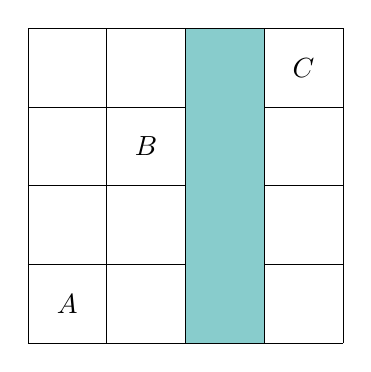
\begin{tikzpicture}
        \draw[step=1cm,black,very thin] (0,0) grid (4,4);
        \draw (0.5,0.5) node{$A$};% the y coordinates of A, B, C could be random
        \draw (1.5,2.5) node{$B$};% but I couldn't get it to work
        \draw (3.5,3.5) node{$C$};
        \filldraw[fill=color4I] (2,0) rectangle (3,4);
    \end{tikzpicture}
    \caption{Illustration for \cref{lem:Rectangle cut}: The path from $A$ to $B$ cannot be made any shorter by entering the rectangle since it could just go along the border. Meanwhile, removing the rectangle makes new paths $A$ to $C$ and $B$ to $C$.}
\end{figure}

\begin{conclusion}
And so, $\#_{1, n} = n$
\end{conclusion}

\begin{proof}
The only piece that could possibly fit is the \pentI~piece, which is removable thanks to \cref{lem:Rectangle cut}.
\end{proof}

\begin{figure}[htbp!]
    \centering
    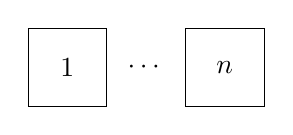
\begin{tikzpicture}
        \draw[step=1cm,black,very thin] (0,0) grid (1,1);
        \draw[step=1cm,black,very thin] (2,0) grid (3,1);
        \draw (0.5,0.5) node{1};
        \draw (1.5,0.5) node{$\cdots$};
        \draw (2.5,0.5) node{$n$};
    \end{tikzpicture}
    \caption{$\#_{1, n} = n$ (where $1 < n$). \cite{sheet}}
\end{figure}





\section{One pentomino}

We know that \cref{lem:Border removal} works for rectangles that span from one side to the other, but this also works for the corner.

\begin{theorem}
\label{th:Corner removal}

A platter $P$ is made of the set of squares $S$ and all squares to the bottom-left of any square in $S$. Then it satisfies \cref{lem:Border removal}.
\end{theorem}

\begin{proof}
Informally, $\adj(P)$ forms a staircase-like shape. So any path along $\adj(P)$ will go in only two cardinal directions, and in fact will have the length of the Manhattan distance between its two endpoints, which cannot be improved upon.
\end{proof}

\begin{note}
This construction may be rotated and reflected.
\end{note}

\begin{theorem}[Cut corner removal]
\label{th:Cut corner removal}

This extends \cref{th:Corner removal} to potentially apply to each ``\badterm{side}'' (i.e.\ subgrid border) of a platter that cuts the grid into subgrids.
\end{theorem}

\begin{proof}
For each subgrid $s$, try applying \cref{th:Corner removal} as if all the other subgrids were part of the platter. Including these other subgrids does not affect $\border(P)_s$, so this is valid for determining whether a path in $s$ can be improved.
\end{proof}

\begin{note}
If \cref{th:Corner removal} applies to the entire border, then as a result the whole platter can be removed, since no path within any of the subgrids can be improved.
\end{note}

\begin{figure}[htbp]
    \centering
    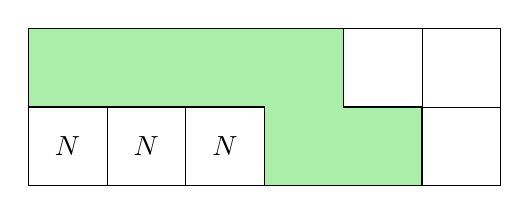
\begin{tikzpicture}
        \draw[step=1cm,black,very thin] (0,0) grid (6,2);
        \draw (0.5,0.5) node{$N$};
        \draw (1.5,0.5) node{$N$};
        \draw (2.5,0.5) node{$N$};
        \filldraw[fill=colorN] (0,1) -- (3,1) -- (3,0) -- (5,0) -- (5,1) -- (4,1) -- (4,2) -- (0,2) -- cycle;
    \end{tikzpicture}
    \caption{Example for \cref{th:Cut corner removal}: \minordetail{The pentomino} \pentN{} divides the grid into two. For the purposes of the subgrid on the right, \pentN{} may as well also include the subgrid on the left (marked with three $N$'s). This new platter satisfies \cref{th:Corner removal}.}
\end{figure}



\subsection{\texorpdfstring{$2 \times n$}{2 \texttimes\ n} grids}

Consider a $2 \times n$ grid. The only pentominoes that fit are \pentI, \pentL, \pentP, \pentN, \pentU, and \pentY.

By \cref{th:Cut corner removal} (Cut corner removal), \pentL, \pentP, \pentN, \pentU, and \pentY{} can be removed from consideration in $2 \times n$ areas, so only \pentI{} is left. While placing \pentI{} on the corner does not help, placing \pentI{} anywhere else increases $\#^p_{2, n}$ by 1 --- the unique way to show $\#_{2, n} = n + 2$ for $n \ge 7$.

\begin{figure}[htbp!]
    \centering
    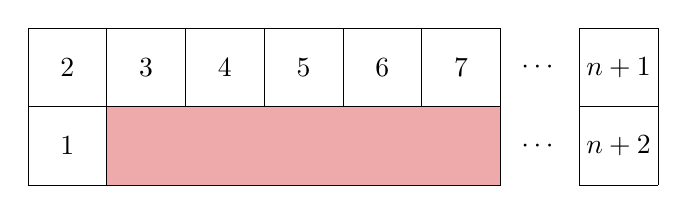
\begin{tikzpicture}
        \draw[step=1cm,black,very thin] (0,0) grid (6,2);
        \draw[step=1cm,black,very thin] (7,0) grid (8,2);
        \draw (0.5,0.5) node{1};
        \draw (0.5,1.5) node{2};
        \draw (1.5,1.5) node{3};
        \draw (2.5,1.5) node{4};
        \draw (3.5,1.5) node{5};
        \draw (4.5,1.5) node{6};
        \draw (5.5,1.5) node{7};
        \filldraw[fill=colorI] (1,0) rectangle (6,1);
        \draw (6.5,0.5) node{$\cdots$};
        \draw (6.5,1.5) node{$\cdots$};
        \draw (7.5,1.5) node{$n + 1$};
        \draw (7.5,0.5) node{$n + 2$};
    \end{tikzpicture}
    \caption{$\#_{2, n} = n + 2$ (where $7 \le n$). \cite{sheet}}
\end{figure}



\subsection{\texorpdfstring{$3 \times n$}{3 \texttimes\ n} grids}

%\begin{definition}[Bound]
%A platter's \newterm{bound} are the squares of its border adjacent to some square that is outside and not part of the border. $\bound(P) = \border(P) \cap \adj(\outside(P) \setminus \border(P))$
%\end{definition}
%
\begin{definition}[Cave]
A subgrid is a \newterm{cave} iff it is only connected to the rest of the subgrid its in by one square. That square is called a \newterm{separating vertex}. \cite{enwiki:separatingvertex}
\end{definition}
%
%\begin{example}[Caves of pentominoes]
%No pentomino has a hole, but there is one with a cave: U (Figure \ref{fig:ucave}). Although, any platter touching the wall has holes.
%\end{example}
%
\begin{figure}
    \centering
    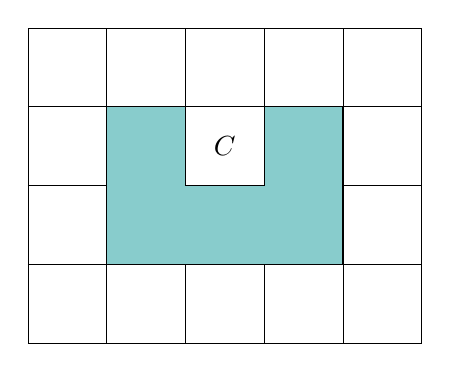
\begin{tikzpicture}
        \draw[step=1cm,black,very thin] (0,0) grid (5,4);
        \filldraw[fill=colorU,shift={(1,1)}] (0,0) -- (3,0) -- (3,2) -- (2,2) -- (2,1) -- (1,1) -- (1,2) -- (0,2) -- cycle;
%        \draw (0.5,0.5) node{$B$};
%        \draw (1.5,0.5) node{$B$};
%        \draw (2.5,0.5) node{$B$};
%        \draw (3.5,0.5) node{$B$};
%        \draw (4.5,0.5) node{$B$};
%        \draw (4.5,1.5) node{$B$};
%        \draw (4.5,2.5) node{$B$};
%        \draw (4.5,3.5) node{$B$};
%        \draw (3.5,3.5) node{$B$};
%        \draw (2.5,3.5) node{$B$};
%        \draw (1.5,3.5) node{$B$};
%        \draw (0.5,3.5) node{$B$};
%        \draw (0.5,2.5) node{$B$};
%        \draw (0.5,1.5) node{$B$};
        \draw (2.5,2.5) node{$C$};
    \end{tikzpicture}
    \caption{\pentU{} is the unique pentomino with a cave square.}
    \label{fig:ucave}
\end{figure}
%
%\begin{definition}[Convex]
%A platter is \newterm{convex} iff it has no caves.
%\end{definition}

\begin{theorem}[Ways to orient a pentomino]
\label{th:Pentomino orientations}

A square has 4 symmetries, so a platter has at most 8 orientations, ignoring location within a grid. However, some pentominoes have one or more symmetries, which reduce the possible orientations (\cref{tab:pentomino orientations}).

    \begin{table}[htbp]
        \centering
        \caption{Number of ways to orient each pentomino. \cite[0:41]{v1}}
        \begin{tabular}{ccc}
            \toprule
            Pentomino & Symmetries & Orientations \\
            \midrule
            \pentX{} & 4 & 1 \\
            \pentI{} & 2 & 2 \\
            \pentT{} & 1 & 4 \\
            \pentU{} & 1 & 4 \\
            \pentV{} & 1 & 4 \\
            \pentW{} & 1 & 4 \\
            \pentZ{} & 1 & 4 \\
            \pentF{} & 0 & 8 \\
            \pentL{} & 0 & 8 \\
            \pentP{} & 0 & 8 \\
            \pentN{} & 0 & 8 \\
            \pentY{} & 0 & 8 \\
            \bottomrule
        \end{tabular}
        \label{tab:pentomino orientations}
    \end{table}
\end{theorem}

\begin{corollary}
\Cref{th:Cut corner removal} works for \pentV, \pentW, \pentZ, the vertical orientations of \pentP, \pentT, and \pentU, and one side of either orientation of \pentF. Note that we may reflect the entire grid itself along both a vertical and horizontal axis, since \cref{th:Cut corner removal} works after reflection. This reduces the number of orientations \minordetail{a pentomino could have} by a factor of four; \minordetail{the maximum orientations goes from eight to two}. (\Cref{fig:Reduced orientations})
\end{corollary}

\begin{note}
\pentU{} satisfies a general version of \cref{th:Cut corner removal} where both corners are covered.
\end{note}

\begin{figure}
    \centering
    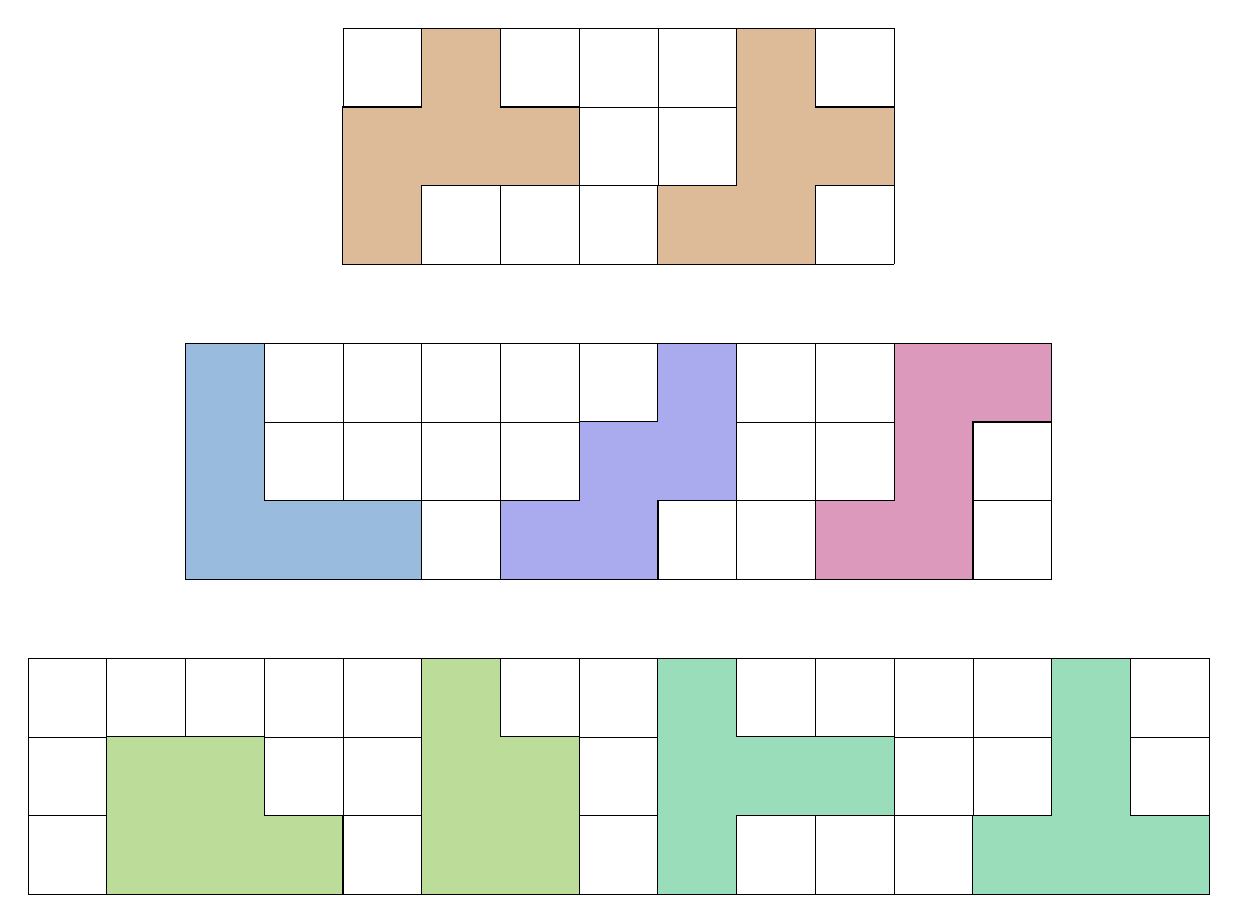
\begin{tikzpicture}
        \begin{scope}[xshift=1cm]
            \draw[step=1cm,black,very thin] (0,0) grid (11,3);
            \filldraw[fill=colorV] (0,0) -- (3,0) -- (3,1) -- (1,1) -- (1,3) -- (0,3) -- cycle;

            \begin{scope}[xshift=4cm]
            \filldraw[fill=colorW] (0,0) -- (2,0) -- (2,1) -- (3,1) -- (3,3) -- (2,3) -- (2,2) -- (1,2) -- (1,1) -- (0,1) -- cycle;
            \end{scope}

            \begin{scope}[xshift=8cm]
            \filldraw[fill=colorZ] (0,0) -- (2,0) -- (2,2) -- (3,2) -- (3,3) -- (1,3) -- (1,1) -- (0,1) -- cycle;
            \end{scope}
        \end{scope}

        \begin{scope}[yshift=-4cm]
            \draw[step=1cm,black,very thin] (-1,0) grid (14,3);
            \filldraw[fill=colorP] (0,0) -- (3,0) -- (3,1) -- (2,1) -- (2,2) -- (0,2) -- cycle;

            \begin{scope}[xshift=4cm]
            \filldraw[fill=colorP] (0,0) -- (0,3) -- (1,3) -- (1,2) -- (2,2) -- (2,0) -- cycle;
            \end{scope}

            \begin{scope}[xshift=7cm]
            \filldraw[fill=colorT] (0,0) -- (0,3) -- (1,3) -- (1,2) -- (3,2) -- (3,1) -- (1,1) -- (1,0) -- cycle;
            \end{scope}

            \begin{scope}[xshift=11cm]
            \filldraw[fill=colorT] (0,0) -- (3,0) -- (3,1) -- (2,1) -- (2,3) -- (1,3) -- (1,1) -- (0,1) -- cycle;
            \end{scope}
        \end{scope}

        \begin{scope}[shift={(3cm,4cm)}]
            \draw[step=1cm,black,very thin] (0,0) grid (7,3);
            \filldraw[fill=colorF] (0,0) -- (1,0) -- (1,1) -- (3,1) -- (3,2) -- (2,2) -- (2,3) -- (1,3) -- (1,2) -- (0,2) -- cycle;

            \begin{scope}[xshift=4cm]
            \filldraw[fill=colorF] (0,0) -- (0,1) -- (1,1) -- (1,3) -- (2,3) -- (2,2) -- (3,2) -- (3,1) -- (2,1) -- (2,0) -- cycle;
            \end{scope}
        \end{scope}
    \end{tikzpicture}
    \caption{All orientations of \pentF, \pentV, \pentW, \pentZ, \pentP, and \pentT{} in a $3 \times n$ after reducing by symmetry. The left side of both \pentF's are ignorable, as well as \minordetail{both sides of} the right \pentP and \pentT. Additionally, the second \pentF{} is strictly worse than the first \pentF, since after filling in the ignorable subgrid, the first \pentF{} practically replaces a wall with an empty square when compared to the second \pentF.}
    \label{fig:Reduced orientations}
\end{figure}

\begin{property}[Cycle inefficiency]
\label{prop:cycineff}

If there is a cycle of empty squares in a grid, the path will not use all empty squares.
\end{property}

\begin{property}[Zero pentomino result]
\label{prop:zeroplace}

With nothing placed, we have $\#^{\emptyset}_{n, m} = n + m - 1$
\end{property}

\begin{property}[One-pentomino solution]
\label{prop:oneplace}

Say we place a pentomino and $n + m - 1, nm - 10 < \#^p_{n, m}$. Then any solution must contain one pentomino.
\end{property}

\begin{lemma}[Maximal solutions in $3 \times n$ grids]
\label{lem:max3x3}

Say we know how many pentominoes are in a solution, and that all squares are used. Then:
\begin{itemize}
    \item \pentF, \pentX, and \pentU{} are not part of the solution.
    \item \pentL, \pentN, and \pentY{} must have their $1 \times 4$ in the middle row, if they are not adjacent to other pentominoes.
\end{itemize}
\end{lemma}

\begin{proof}
First, we take \pentU{} from the first bullet point. If a path enters \minordetail{or exits} a cave square \minordetail{(enters without loss of generality)}, it cannot exit since there is only one entrance. Since \pentU{} has a cave square, we can say a path must end there. But if \pentU{} is placed horizontally (2 rows by 3 columns, \cref{fig:u3x4}), it is at least as good to just go around the \pentU{} (removing any obstacles).
\begin{itemize}
    \item Pentominoes must be placed so that the grid is \emph{not} split into two. This is impossible for \pentF{} and \pentX{}, which span a $1 \times 3$ area with two squares padding each side of the $1 \times 3$, forcing the $1 \times 3$ into the center.
    \item If a pentomino that spans a $1 \times 4$ area (\pentL, \pentN, \pentY) has their $1 \times 4$ on the edge of the grid, there are two disjoint $2 \times 2$ cycles (\cref{fig:1x4in3x4}) which cannot be prevented by the remaining square of the pentomino and no help from other pentominoes. But this is not allowed by \cref{prop:cycineff}.\qedhere
\end{itemize}
\end{proof}

\begin{figure}
    \centering
    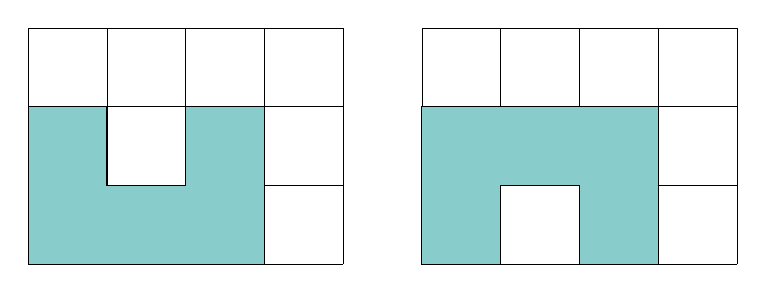
\begin{tikzpicture}
        \draw[step=1cm,black,very thin] (0,0) grid (4,3);
        \filldraw[fill=colorU] (0,0) -- (3,0) -- (3,2) -- (2,2) -- (2,1) -- (1,1) -- (1,2) -- (0,2) -- cycle;

        \begin{scope}[xshift=5cm]
            \draw[step=1cm,black,very thin] (0,0) grid (4,3);
            \filldraw[fill=colorU] (0,0) -- (1,0) -- (1,1) -- (2,1) -- (2,0) -- (3,0) -- (3,2) -- (0,2) -- cycle;
        \end{scope}
    \end{tikzpicture}
    \caption{Horizontal orientations of \pentU{} in a $3 \times 4$ (footnote: \protect\footnotemark)}
    \label{fig:u3x4}
\end{figure}

\footnotetext{film2860 on discord used gpt-4o to try to remove pixel artifacts. It generated equivalent code, which did not fix the problem, but did illustrate the usage of scopes which was helpful as a beginner. So congrats on contributing!}

\begin{figure}
    \centering
    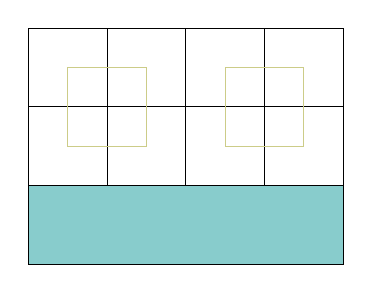
\begin{tikzpicture}
        \draw[step=1cm,black,very thin] (0,0) grid (4,3);
        \filldraw[fill=color4I] (0,0) rectangle (4,1);
        \draw[color4O] (0.5,1.5) rectangle (1.5,2.5);
        \draw[color4O] (2.5,1.5) rectangle (3.5,2.5);
    \end{tikzpicture}
    \caption{Two disjoint $2 \times 2$ cycles existing after placing a $1 \times 4$ on the edge of a $3 \times 4$.}
    \label{fig:1x4in3x4}
\end{figure}

\begin{figure}[htbp!]
    \centering
    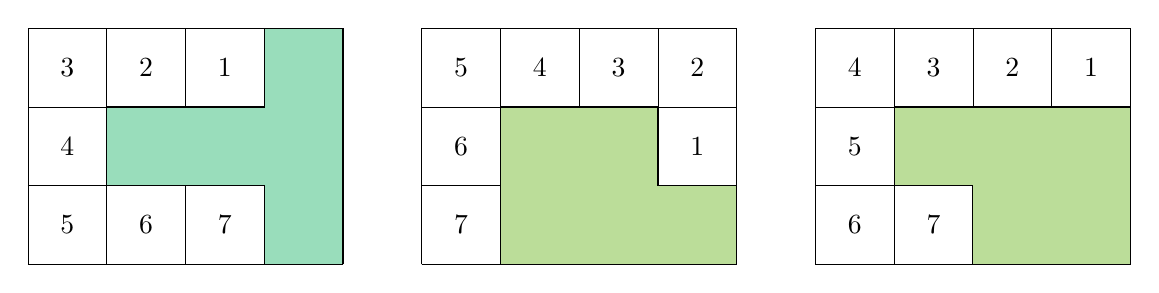
\begin{tikzpicture}
        \draw[step=1cm,black,very thin] (0,0) grid (4,3);
        \draw (2.5,2.5) node{1};
        \draw (1.5,2.5) node{2};
        \draw (0.5,2.5) node{3};
        \draw (0.5,1.5) node{4};
        \draw (0.5,0.5) node{5};
        \draw (1.5,0.5) node{6};
        \draw (2.5,0.5) node{7};
        \filldraw[fill=colorT] (3,0) -- (4,0) -- (4,3) -- (3,3) -- (3,2) -- (1,2) -- (1,1) -- (3,1) -- cycle;

        \begin{scope}[xshift=5cm]
            \draw[step=1cm,black,very thin] (0,0) grid (4,3);
            \draw (3.5,1.5) node{1};
            \draw (3.5,2.5) node{2};
            \draw (2.5,2.5) node{3};
            \draw (1.5,2.5) node{4};
            \draw (0.5,2.5) node{5};
            \draw (0.5,1.5) node{6};
            \draw (0.5,0.5) node{7};
            \filldraw[fill=colorP] (1,2) -- (1,0) -- (4,0) -- (4,1) -- (3,1) -- (3,2) -- cycle;
        \end{scope}

        \begin{scope}[xshift=10cm]
            \draw[step=1cm,black,very thin] (0,0) grid (4,3);
            \draw (3.5,2.5) node{1};
            \draw (2.5,2.5) node{2};
            \draw (1.5,2.5) node{3};
            \draw (0.5,2.5) node{4};
            \draw (0.5,1.5) node{5};
            \draw (0.5,0.5) node{6};
            \draw (1.5,0.5) node{7};
            \filldraw[fill=colorP] (1,2) -- (1,1) -- (2,1) -- (2,0) -- (4,0) -- (4,2) -- cycle;
        \end{scope}
    \end{tikzpicture}
    \caption{$\#_{3, 4} = 7$. \cite[6:04]{v2}}
    \label{fig:3x4}
\end{figure}

\begin{theorem}
$\#_{3, 4} = 7$
\end{theorem}

\begin{proof}
By \cref{fig:3x4}, we have maximal solutions with 1 pentomino, and since $3 + 4 - 1, 12 - 10 < 7$, \cref{lem:max3x3} applies. \pentL, \pentN, and \pentY{} can be eliminated since a $1 \times 4$ in the center row would divide the grid into two subgrids (this is not allowed; remember that every nonempty square must be in the path).

We are left with \minordetail{the pentominoes} \pentP{} and \pentT{}. If \pentP{} does not touch the corner, after placing the $2 \times 2$, the 5th square must divide the grid in two. There are four ways to touch the corner, and two work. For \pentT, there is only one orientation that does not cut the grid. So the three solutions given by \cite[6:04]{v2} are the only ones.
\end{proof}

A polynomial's \badterm{contribution} is informally how much longer it makes a given path. But \cref{fig:nontrivialcontribution} shows a formal definition is still a ways away. In such examples, we must consider entire platters.

\begin{figure}[htbp]
    \centering
    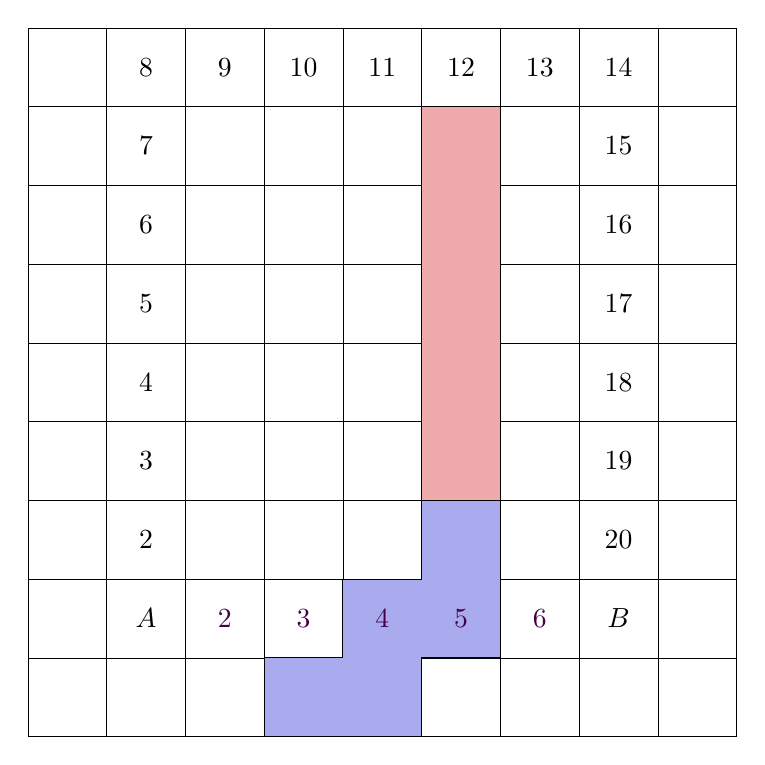
\begin{tikzpicture}
        \draw[step=1cm,black,very thin] (0,0) grid (9,9);
        \draw (1.5,1.5) node{$A$};
        \draw (1.5,2.5) node{2};
        \draw (1.5,3.5) node{3};
        \draw (1.5,4.5) node{4};
        \draw (1.5,5.5) node{5};
        \draw (1.5,6.5) node{6};
        \draw (1.5,7.5) node{7};
        \draw (1.5,8.5) node{8};
        \draw (2.5,8.5) node{9};
        \draw (3.5,8.5) node{10};
        \draw (4.5,8.5) node{11};
        \draw (5.5,8.5) node{12};
        \draw (6.5,8.5) node{13};
        \draw (7.5,8.5) node{14};
        \draw (7.5,7.5) node{15};
        \draw (7.5,6.5) node{16};
        \draw (7.5,5.5) node{17};
        \draw (7.5,4.5) node{18};
        \draw (7.5,3.5) node{19};
        \draw (7.5,2.5) node{20};
        \filldraw[fill=colorI] (5,3) rectangle (6,8);
        \filldraw[fill=colorW] (3,0) -- (3,1) -- (4,1) -- (4,2) -- (5,2) -- (5,3) -- (6,3) -- (6,1) -- (5,1) -- (5,0) -- cycle;
        \draw (2.5,1.5) node{\textcolor{colorSecondary}{2}};
        \draw (3.5,1.5) node{\textcolor{colorSecondary}{3}};
        \draw (4.5,1.5) node{\textcolor{colorSecondary}{4}};
        \draw (5.5,1.5) node{\textcolor{colorSecondary}{5}};
        \draw (6.5,1.5) node{\textcolor{colorSecondary}{6}};
        \draw (7.5,1.5) node{$B$};
    \end{tikzpicture}
    \caption{If the I pentomino was already placed, then adding the \pentW{} changes the path's length from 7 to 21. Nevertheless, \pentW's contribution $C($\pentW$) = 4$. Additionally, \pentW{} helps by blocking the bottom row. So some squares are spent on setup, and some on lengthening the path.}
    \label{fig:nontrivialcontribution}
\end{figure}

% \subsection{How to add Comments and Track Changes}

% Comments can be added to your project by highlighting some text and clicking ``Add comment'' in the top right of the editor pane. To view existing comments, click on the Review menu in the toolbar above. To reply to a comment, click on the Reply button in the lower right corner of the comment. You can close the Review pane by clicking its name on the toolbar when you're done reviewing for the time being.

% \subsection{How to add Lists}

% You can make lists with automatic numbering \dots

% \begin{enumerate}
% \item Like this,
% \item and like this.
% \end{enumerate}
% \dots or bullet points \dots
% \begin{itemize}
% \item Like this,
% \item and like this.
% \end{itemize}


% \subsection{How to change the margins and paper size}

% Usually the template you're using will have the page margins and paper size set correctly for that use-case. For example, if you're using a journal article template provided by the journal publisher, that template will be formatted according to their requirements. In these cases, it's best not to alter the margins directly.

% If however you're using a more general template, such as this one, and would like to alter the margins, a common way to do so is via the geometry package. You can find the geometry package loaded in the preamble at the top of this example file, and if you'd like to learn more about how to adjust the settings, please visit this help article on \href{https://www.overleaf.com/learn/latex/page_size_and_margins}{page size and margins}.

% \subsection{How to change the document language and spell check settings}

% Overleaf supports many different languages, including multiple different languages within one document.

% To configure the document language, simply edit the option provided to the babel package in the preamble at the top of this example project. To learn more about the different options, please visit this help article on \href{https://www.overleaf.com/learn/latex/International_language_support}{international language support}.

% To change the spell check language, simply open the Overleaf menu at the top left of the editor window, scroll down to the spell check setting, and adjust accordingly.

% \subsection{Good luck!}

% We hope you find Overleaf useful, and do take a look at our \href{https://www.overleaf.com/learn}{help library} for more tutorials and user guides! Please also let us know if you have any feedback using the Contact Us link at the bottom of the Overleaf menu --- or use the contact form at \url{https://www.overleaf.com/contact}.

\FloatBarrier
\printbibliography

\end{document}